\documentclass[12pt,a4paper]{report}
\usepackage{cite}
\usepackage{longtable}
\usepackage[dvips]{graphicx,color}
\usepackage{makeidx}
\usepackage{nomencl}
\usepackage{float}
\usepackage{amsmath}
\usepackage{graphicx}
\usepackage{amssymb}
\usepackage{multicol}
\usepackage{dsfont}
\usepackage[bottom]{footmisc}
\usepackage{subfigure}
\usepackage[OT2,OT1]{fontenc}
\newcommand{\imsize}{3in}
\newcommand{\norm}[1]{\left|\left|#1\right|\right|}
\newtheorem{definition}{Definition}
\newtheorem {remark}{Remark}
\newtheorem{thm}{Theorem}
\setlength{\textwidth}{6.3in}
\setlength{\textheight}{8.8in}
\addtolength{\oddsidemargin}{-0.5in}
\addtolength{\topmargin}{-0.2in}
\usepackage{tikz}
\usetikzlibrary{shapes,arrows,chains,matrix,positioning,scopes,decorations.pathmorphing,shadows,calc}

\begin{document}
\title{
	\textbf
	{\LARGE{Multilevel Inverter Based on Switched-Capacitance Structure}}\\ 
	}
\author{
	{\Large{INTERIM PROJECT REPORT}} \\
	{\large{Submitted by}}\vspace{.25in}\\	
	{\bf\large ABHILASH M M (TCR15EE002)} \\
	{\bf\large ALIN ANTO (TCR15EE016)} \\
	{\bf\large DEVIKA SAJEEV (TCR15EE042)} \\
	{\bf\large DON DEV (TCR15EE046)}\vspace{0.25in} \\
	to\\
	The APJ Abdul Kalam Technological University\\
	in partial fulfillment of the requirements for the award of the degree\\
	of\\
	Bachelor of Technology\\
	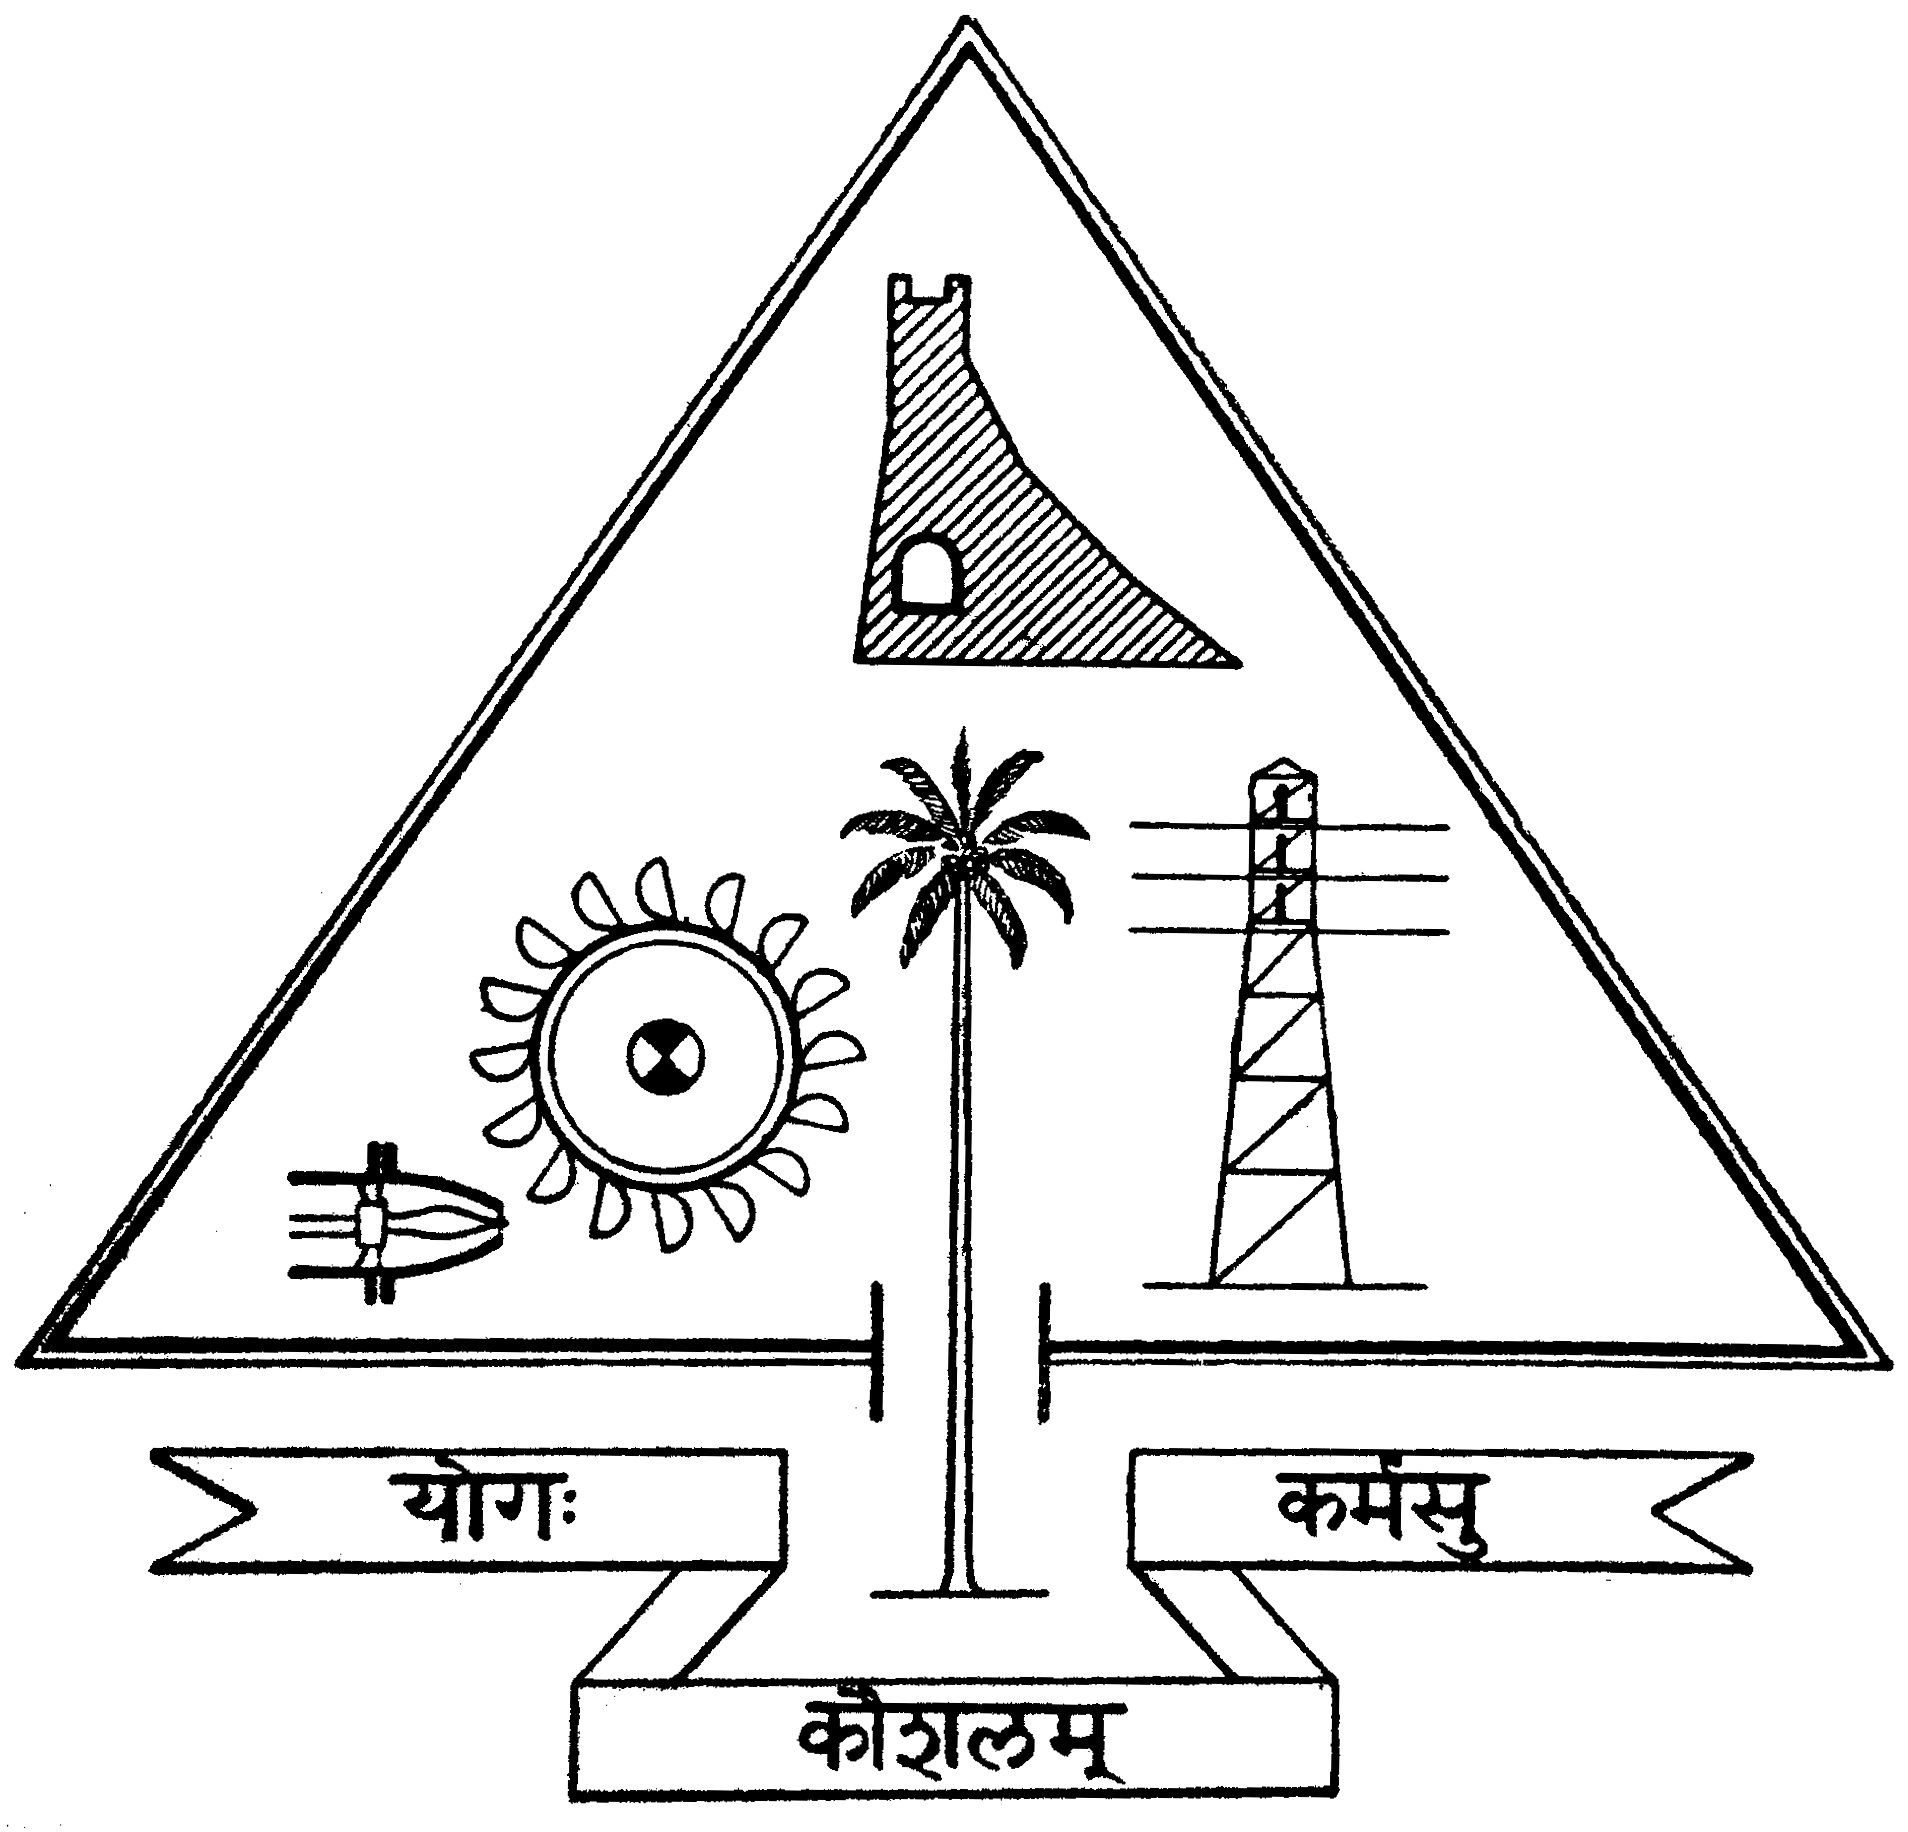
\includegraphics[height=1.4in, width=1.4in]{figures/gectemblem}\\
	Department of Electrical Engineering \\
	Government Engineering College  \\
}
\date{FEBRUARY - 2019}
\maketitle

\begin{abstract}
Multilevel inverter is a power electronic device capable of providing desired output using multiple lower level DC voltages as an input. Multilevel inverters are gaining popularity over conventional two level inverters because it can produce a smoother stepped output waveform. Moreover, the output obtained from multilevel inverters has lower $d_v/d_t$ and lower harmonic distortions. Multilevel inverters usually make use of diode clamped, flying capacitor or cascaded H-bridge topologies. These topologies suffer from disadvantages such as multitude of components, large size and cost as well as complex control. This project aims to use a switched-capacitance (SC) structure to overcome the disadvantages of the existing topologies. It involves adding an SC structure to the H-bridge inverter using capacitors, switches and diodes to create a multilevel DC voltage at the DC bus of the H-bridge circuit. The proposed technology will improve upon the existing technology by having boost operation without magnetic elements, fewer components, less complex control and using only one power DC source. This project work involves the simulation and hardware implementation of Switched Capacitance Multilevel Inverter
\end{abstract}

	\pagenumbering{arabic}
\clearpage
\section*{Introduction}
\hspace{0.2cm} Recently, multilevel inverters (MIs) are getting more attention from researchers because of advantages like better waveform quality, lower EM noise, and lower device stress. MIs are used to couple a DC source to an AC bus for applications like electric motor drivers, uninterruptible power supplies, and distributed generation systems. The following topologies are now used in practice:-\\

\noindent1$)$Neutral-point clamped (Diode clamped).\\
2$)$Flying capacitor.\\
3$)$Cascaded H-bridge (CHB).\\

\noindent For low-power applications, the system size and cost are the main concerns.
Problems in multilevel inverters (MIs) employing current topologies are the following:-\\

\noindent1$)$Large number of components( switches, power supplies, capacitors, and diodes).\\
2$)$Large size and high cost.\\
3$)$Complex control.\\

\noindent Solution to the problem is a new MI topology that uses a Switched Capacitor(SC) structure in cascade with an H-bridge. The objective of this new system is to achieve the following characteristics for a  SC-MI:-\\

\noindent1$)$Fewer components(switches, sources and capacitors).\\
2$)$Smaller and less expensive.\\
3$)$Less complex control.\\
4$)$Requires only one power DC source.\\
5$)$Boost operation without magnetic elements.\\
	
\begin{center}
	\begin{tabular}{|c|c|} 
		\hline
		{\bf Hardware Requirements} & {\bf Software Requirements} \\  
		\hline
		DSO (Analysis) & Matlab (Simulation) \\ 
		\hline
		DSP (controller) & Proteus (Design) \\
		\hline
		Function generator (Analysis and reference) & Latex (Documentation) \\
		\hline
	\end{tabular}
\end{center}
	
\clearpage

\section*{Methodology}

 \begin{center}
 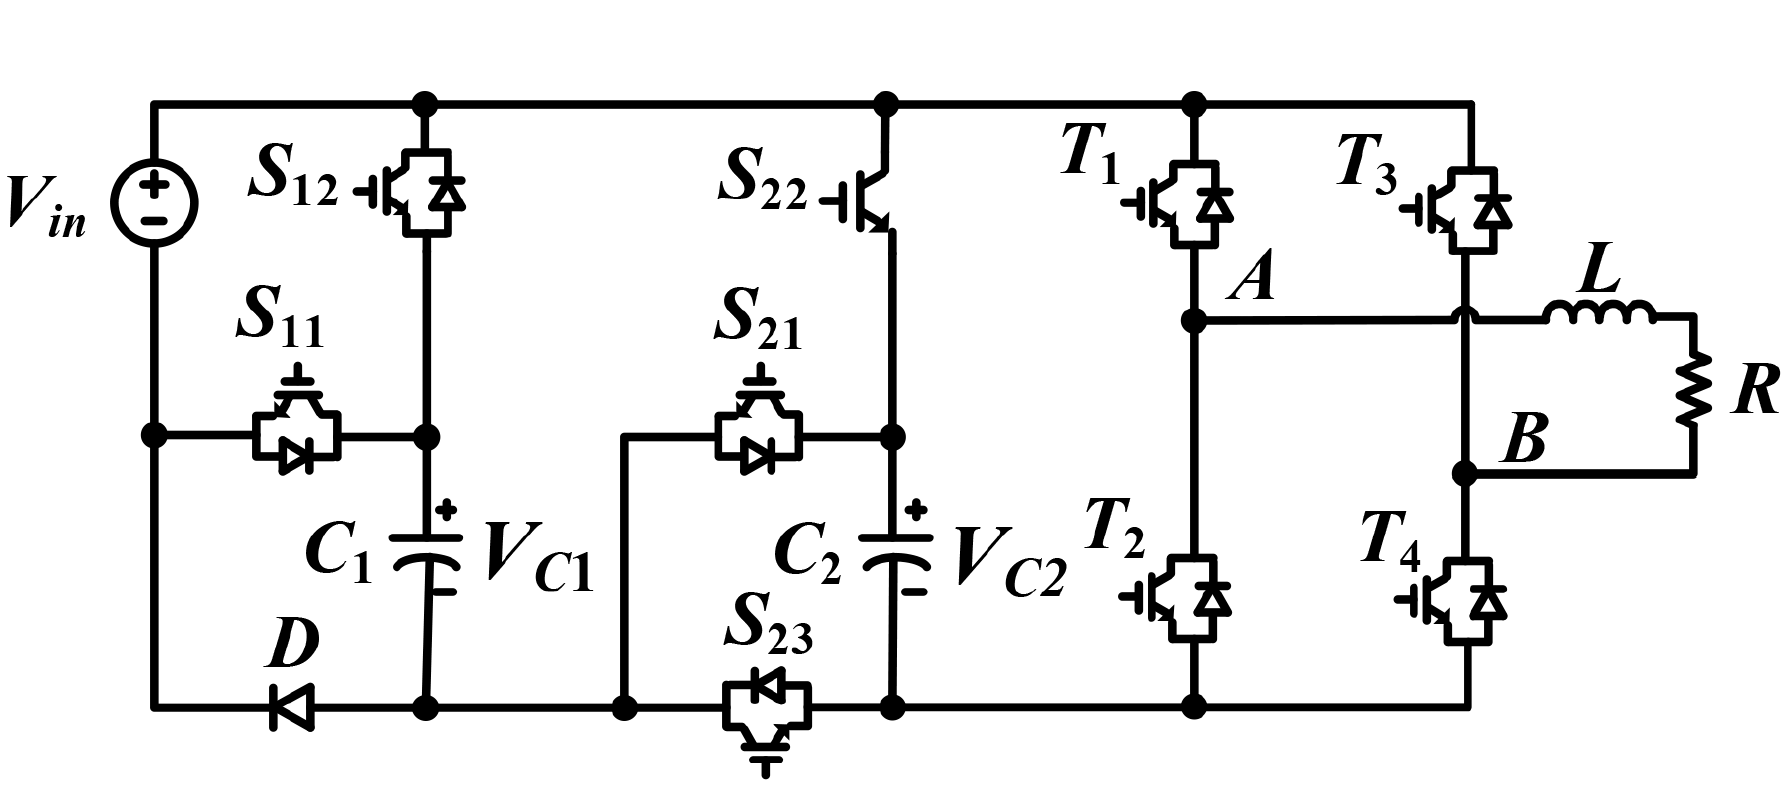
\includegraphics[width=11.5cm,height=5cm]{figures/Main_Circuit}
 \end{center}

 \hspace{0.2cm} The proposed inverter consists of a single DC source, two SC cells connected in parallel with the H-bridge circuit and a load. The first SC cell is a combination of one capacitor, one diode, and two switches ($C_1-D-S_{11}-S_{12}$), and the second SC cell includes one capacitor, and three switches ($C_2-S_{21}-S_{22}-S_{23}$).\\
  
\subsection*{Working}

Capacitor $C_1$ is charged while connected in parallel with the input source through $S_{12}$. It is discharged in series with the input source through $S_{11}$. Capacitor $C_2$ is charged in parallel from the input source and capacitor $C_1$ through $S_{22}$ and $S_{23}$. It is discharged in series with capacitor $C_1$ and the input source through $S_{21}$. $C_1$ is thus charged to $V_{in}$ and $C_2$ is charged to $2V_{in}$. Four Levels of voltage (in addition to a zero level) are therefore obtained by the following combinations:-\\

\begin{center}
	\begin{tabular}{|c|c|c|} 
		\hline
		{\bf MODE} & {\bf OUTPUT VOLTAGE} & {\bf STATE} \\  
		\hline
		1 & $V_{in}$  & Source and $C_1$ in parallel. \\ 
		\hline
		2 & $2V_{in}$ & Source and $C_1$ in series which is then parallel with $C_2$. \\
		\hline
		3 & $3V_{in}$ & Source and $C_1$ in parallel which is then series with $C_2$. \\
		\hline
		4 & $4V_{in}$ & Source, $C_1$ and $C_2$ all in series. \\
		\hline
	\end{tabular}
\end{center}

These four levels of voltage can be reversed in polarity at the output by the H-Bridge. Therefore there are 9 different voltage levels $(4*2 + 1)$ available at the output of the inverter. The switching states are controlled by Phase disposition PWM (PD-PWM).

\clearpage

\subsection*{Modes of Operation}

\begin{center}
	\includegraphics[width=16.5cm,height=10cm]{figures/Mode}
\end{center}

\begin{center}
	\begin{tabular}{|c|c|c|c|c|c|c|c|} 
		\hline
		{\bf MODE} & {\bf OUTPUT VOLTAGE} & {\bf $D$} & {\bf $S_{11}$} & {\bf $S_{12}$} & {\bf $S_{23}$} & {\bf $S_{22}$} & {\bf $S_{21}$} \\  
		\hline
		1 & $V_{in}$  & ON  & OFF & ON  & ON  & ON  & OFF \\ 
		\hline
		2 & $2V_{in}$ & OFF & ON  & OFF & ON  & ON  & OFF \\
		\hline
		3 & $3V_{in}$ & ON  & OFF & ON  & OFF & OFF & ON \\
		\hline
		4 & $4V_{in}$ & OFF & ON  & OFF & OFF & OFF & ON \\
		\hline
	\end{tabular}
\end{center}

\begin{center}
	\begin{tabular}{|c|c|c|} 
		\hline
		{\bf MODE} & {\bf OUTPUT VOLTAGE} & {\bf STATE} \\  
		\hline
		1 & $V_{in}$  & Source and $C_1$ in parallel. \\ 
		\hline
		2 & $2V_{in}$ & Source and $C_1$ in series which is then parallel with $C_2$. \\
		\hline
		3 & $3V_{in}$ & Source and $C_1$ in parallel which is then series with $C_2$. \\
		\hline
		4 & $4V_{in}$ & Source, $C_1$ and $C_2$ all in series. \\
		\hline
	\end{tabular}
\end{center}

In the positive half cycle $T_1$ and $T_4$ are fully turned on whereas $T_2$ and $T_3$ are fully turned OFF. Similarly, in the negative period, $T_2$ and $T_3$ are fully turned on whereas $T_1$ and $T_4$ are fully turned OFF and the components of the SC cells are similar to those in the positive period. To acheive zero voltage output $T_1$ and $T_3$ are turned on simultaneously.

\clearpage

\section*{Simulation}

\begin{center}
	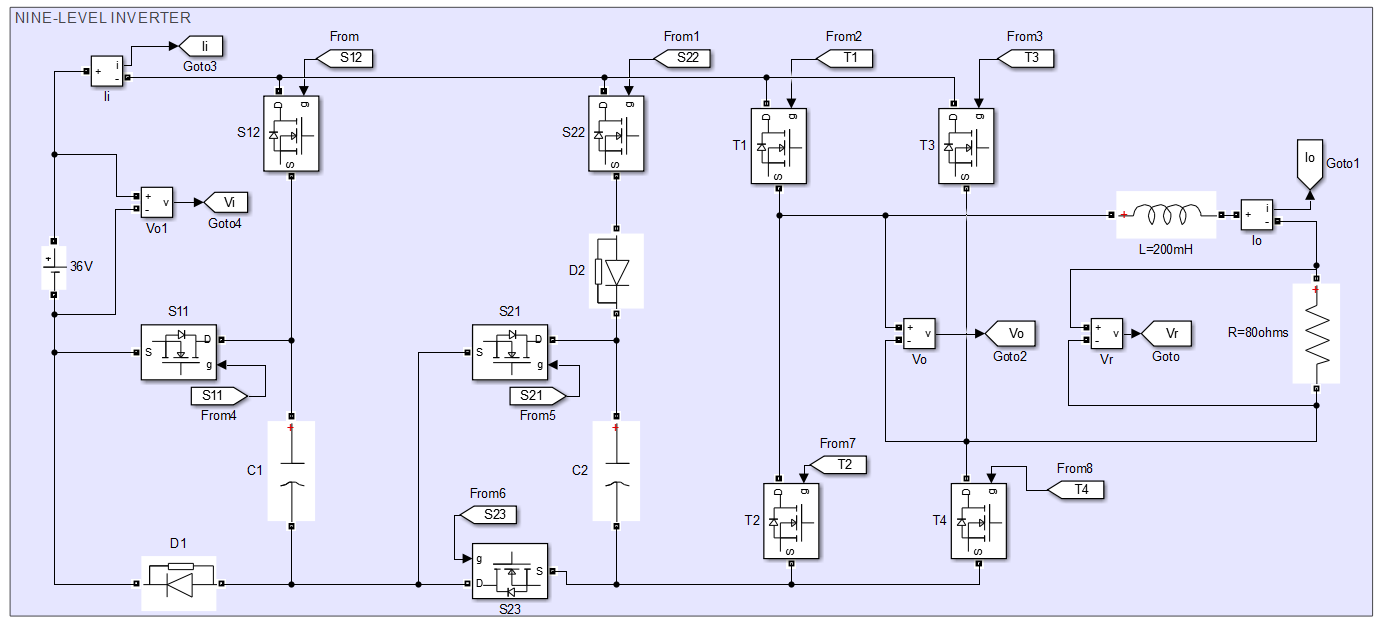
\includegraphics[width=16cm,height=8cm]{figures/SIMULINK_CIRCUIT}
\end{center}

The simulation of the NINE-LEVEL INVERTER was done using the simulink tool in matlab.
Operation of the inverter was verified with R and R-L load. Gating pulses are derived using PD-PWM technique. The switching delay and gate delay are neglected. The design consideration are given in the table below. 

\begin{center}
	\begin{tabular}{|c|c|} 
		\hline
		{\bf PARAMETER} & {\bf VALUE} \\  
		\hline
		$V_{in}$ & $36V$ \\ 
		\hline
		$C_1$ , $C_2$ & $2000{\mu}F $\\
		\hline
		$R + jX_l$ & 80 ${\Omega} + j60{\Omega}$ \\
		\hline
		Diode Forward Drop & $0.7V$ \\
		\hline
		Mosfet On Resistance & $0.1{\Omega}$ \\
		\hline
		Modulating Frequency & $50H_z$ \\
		\hline
		Carrier Frequency & $5000H_z$ \\
		\hline
		Modulating index & $100\%$ \\
		\hline
		
		
	\end{tabular}
\end{center}

\section*{Result}

\begin{center}
	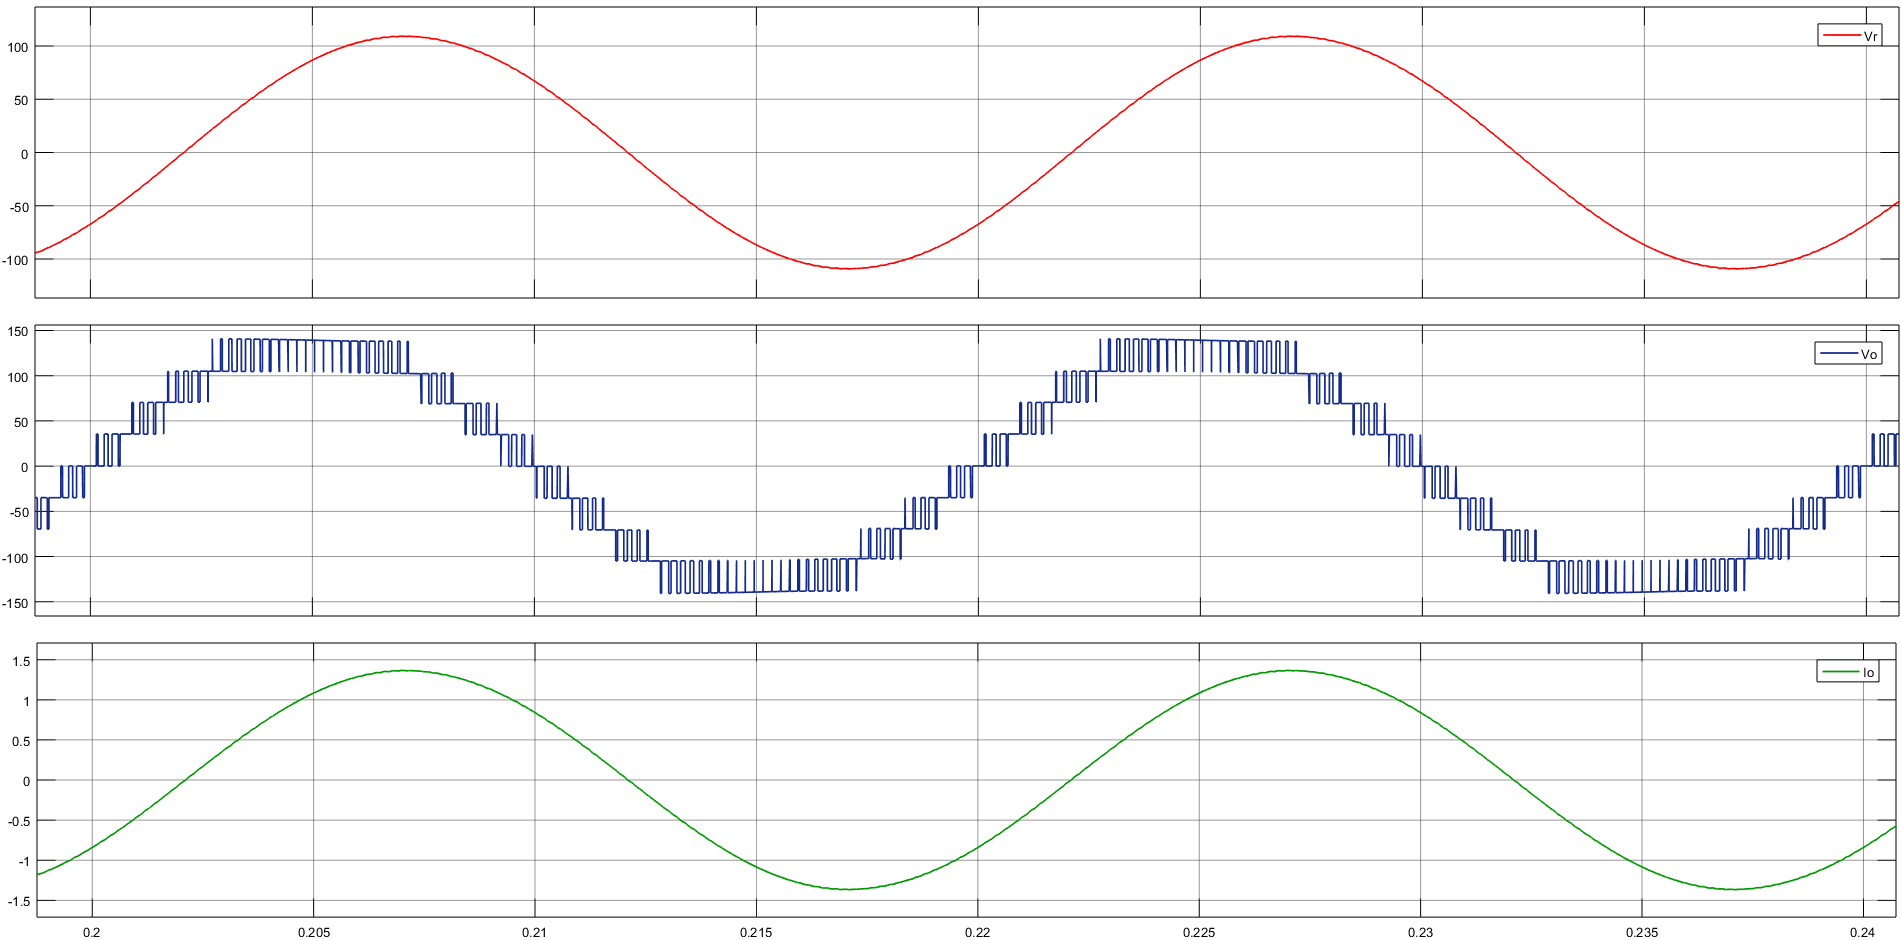
\includegraphics[width=16cm,height=8cm]{figures/SIMULINK_OUTPUT}
\end{center}

The Total Harmonic Distortion in Current was found to be 0.3358\%. Efficiency of the inverter is 95.27\%.


\begin{center}
	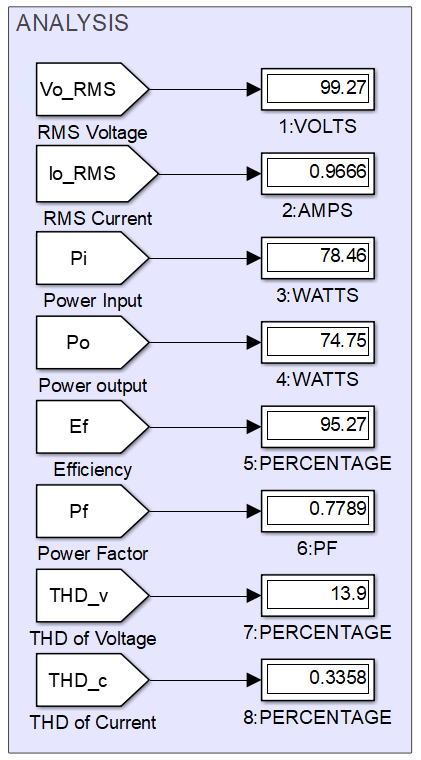
\includegraphics[width=7cm,height=12cm]{figures/SIMULINK_ANALYSIS}
\end{center}


\clearpage

\section*{References}

\noindent[1] {\bf Bac-Bien Ngo}, {\bf Minh-Khai Nguyen} , {\bf Jae-Hong Kim2} and {\bf Firuz Zare}, “\textit{Single-phase multilevel inverter based on switched-capacitor structure}”, IET Power Electron, June 2018, ISSN 1755-4535\\

\noindent[2] {\bf Barry W Williams}, “\textit{Principles and Elements of Power Electronics Devices, Drivers, Applications, and Passive Components}”, 2006, ISBN 978-0-9553384-0-3\\

\noindent[3] {\bf Yuanmao Ye}, {\bf K. W. E. Cheng}, {\bf Junfeng Liu and Kai Ding}, “\textit{A Step-Up Switched-Capacitor Multilevel Inverter With Self-Voltage Balancing}”, IEEE Trans. Ind. Electron, Vol. 61, No. 12, December 2014\\

\noindent[4] {\bf Bhagyalakshmi P S}, {\bf Beena M Varghese} and {\bf Dr. Bos Mathew Jos}, “\textit{Switched Capacitor Multilevel Inverter With Different Modulation Techniques}”, International Conference on Innovations in information Embedded and Communication Systems, 2017\\


	

\end{document}

